\section{Theorie}
\label{sec:theorie}

\subsection{Das Sagnac Interferometer}
\label{sec:theorie_das_sagnac_interferometer}
Abbildung~\ref{fig:aufbau} zeigt den Aufbau des Sagnac Interferometers. Der
Strahl eines Helium-Neon-Lasers ($\lambda=\SI{632.8}{\nano\metre}$) wird über
zwei Spiegel auf den Eingang des Interferometers gelenkt. Dort trifft dieser
senkrecht auf einen polarisierenden Strahlteiler. Während ein Teil des Strahls
den Strahlteiler auf geradem Weg passiert, wird der andere Teil im rechten
Winkel reflektiert. Die zwei Teilstrahlen sind nach Austritt aus dem
Strahlteiler senkrecht zueinander polarisiert. Der Strahlteiler selbst besteht
aus zwei Prismen mit dreieckiger Grundfläche, die auf ihren Hypothenusen
miteinander verbunden sind. Der Normalenvektor der Hypothenusenfläche steht
im~$\SI{45}{\degree}$ Winkel zum einfallenden und reflektierten Strahl. Die zwei
Strahlen laufen nun über drei Spiegel in einem Rechteck, wobei sie sich dabei
überlagern. Danach treffen sie erneut auf den Strahlteiler und verlassen das
Interferometer in Richtung einer Messvorrichtung bestehend aus zwei Photodioden.

Durch vorsichtiges Verschieben des Spiegels vor dem Eingang des Interferometers,
kann der überlagerte Strahl im Interferometer in zwei entgegengesetzt laufende
Strahlen räumlich getrennt werden. Es besteht nun die Möglichkeit ein optisches
Element in einen der beiden Teilstrahlen zu stellen, ohne den anderen Teilstrahl
zu beeinflussen. Ein weiterer Vorteil des Sagnac Interferometers ist, dass es
unempfindlich gegenüber kleineren Erschütterungen ist, da beide Strahlen die
gleiche Wegstrecke durchlaufen.
\begin{figure}[htb]
  \centering
  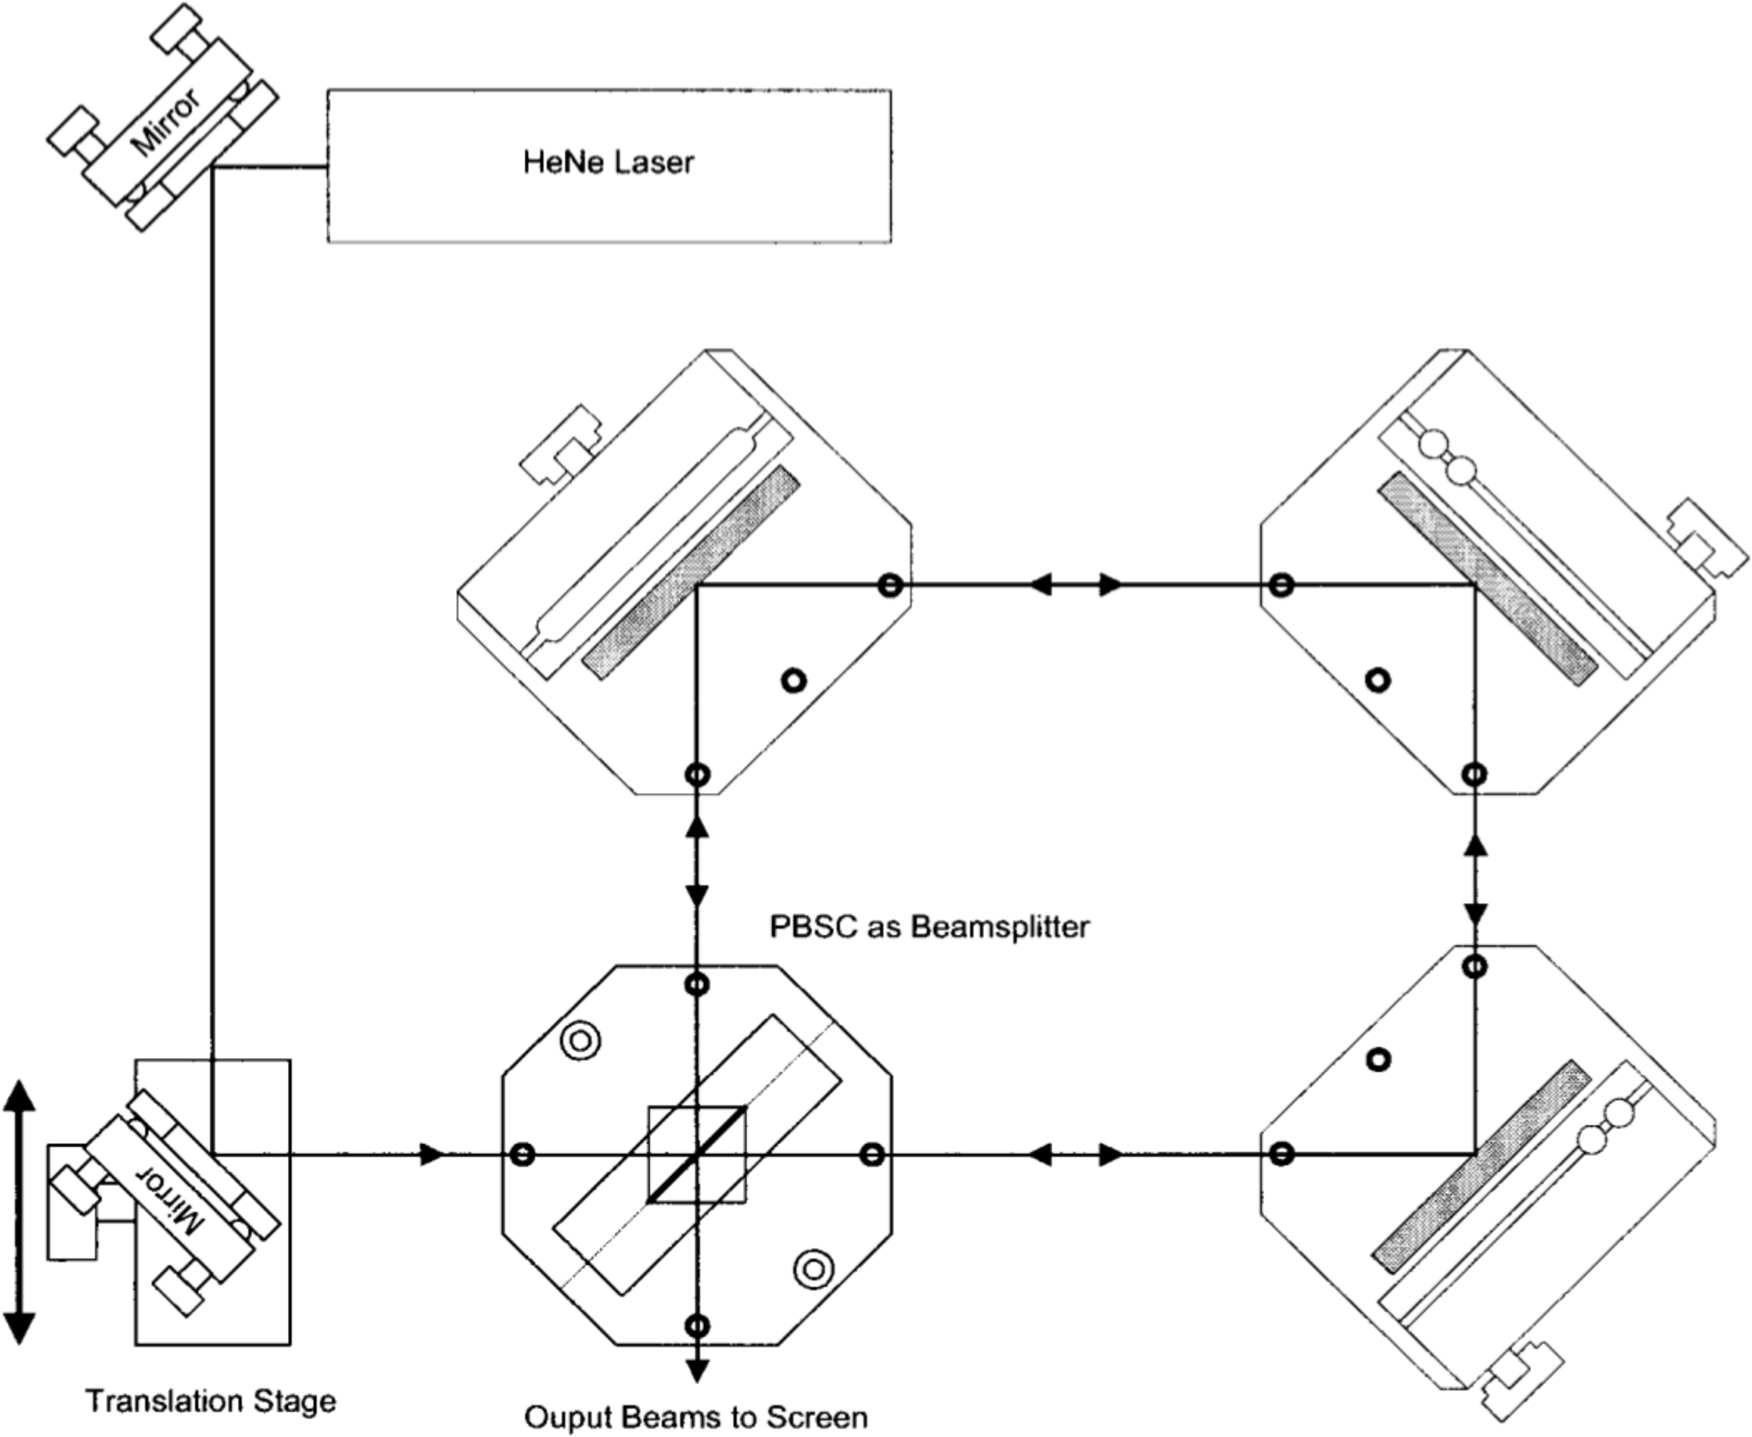
\includegraphics[width=0.8\textwidth]{figures/aufbau.pdf}
  \caption{Aufbau des verwendeten Sagnac Interferometers~\cite{V64}.}
  \label{fig:aufbau}
\end{figure}

\subsection{Kontrast des Sagnac Interferometers}
Der Kontrast eines Interferometers ist gegeben durch
\begin{equation}
  K=\frac{I_{\text{max}}-I_{\text{min}}}{I_{\text{max}}+I_{\text{min}}}.
  \label{eq:kontrast}
\end{equation}
Hierbei bezeichnet~$I_{\text{max}}$ die Intensität eines Interferenzmaximums
und~$I_{\text{min}}$ die Intensität eines Interferenzminimums. Im Idealfall
ist~$I_{\text{min}}=0$ und somit~$K=1$. Im schlechtesten Fall ist kein
Unterschied in der Intensität zwischen Maxima und Minima zu erkennen. Dann
gilt~$I_{\text{max}}=I_{\text{min}}$ und somit~$K=0$.

Im durchgeführten Experiment wird der Kontrast in Abhängigkeit der Einstellung
eines im Strahlgang befindlichen Polarisationsfilters gemessen. Ausgedrückt
durch einen Polarisationswinkel~$\varphi$, einem Phasenwinkel~$\delta$ und einer
Amplitude~$A$ beträgt der Kontrast
\begin{equation}
  K=A\lvert\sin\left(2\varphi+\delta\right)\rvert,
  \label{eq:kontrast}
\end{equation}

\subsection{Bestimmung des Brechungsindex eines Gases}
Der Brechungsindex~$n$ von Materie ist definiert als Quotient der
Lichtgeschwindigkeit im Vakuum und der Lichtgeschwindigkeit in der Materie.
Daraus folgt für die Wellenzahl~$k$ des Lichts in Materie
\begin{equation}
  k=\frac{2\pi}{\lambda_{\text{vac}}}n
\end{equation}
wobei~$\lambda_{\text{vac}}$ die Wellenlänge des Lichts im Vakuum ist.

Für die Bestimmung des Brechungsindex eines Gases wird nun eine Gaszelle der
Länge~$L$ in einem(!) Strahl des Interferometers platziert. Durch die leicht
unterschiedliche Geschwindigkeit des Lichts in der Gaszelle, kommt es zu einer
Phasendifferenz zwischen den beiden Strahlen
\begin{equation}
  \Delta\varphi=\frac{2\pi L}{\lambda_{\text{vac}}}\Delta n,
\end{equation}
die linear mit der Differenz der Brechungsindices des Gases und der
Umgebungsluft zusammenhängt. Durch Überlagerung der beiden Strahlen ergibt sich
ein Interferenzmuster. Die Anzahl~$M$ der beobachteten Interferenzmaxima ist
proportional zur Phasendifferenz. Es gilt
\begin{gather}
  M=\frac{\Delta\varphi}{2\pi}=\frac{L}{\lambda_{\text{vac}}}(n-1) \\
  \shortintertext{und somit}
  n=\frac{\lambda_{\text{vac}}}{L}M+1.
  \label{eq:brechungsindex_gas}
\end{gather}
wobei die Annahme gemacht wurde, dass für den Brechungsindex der
Umgebungsluft~$n_{\text{Luft}}=1$ gilt. Im Allgemeinen ist der Brechungsindex
temperatur- und druckabhängig. Einen Zusammenhang liefert die
Lorentz-Lorenz-Gleichung
\begin{equation}
  \frac{n^2-1}{n^2+2}=\frac{4\pi}{3}N\alpha=\frac{Ap}{RT}
\end{equation}
mit der Polarisierbarkeit~$\alpha$, der Anzahl~$N$ der Moleküle im
Einheitsvolumen, der molaren Refraktivität~$A$, der universellen
Gaskonstante~$R$, sowie Druck~$p$ und Temperatur~$T$. Für Gase liegt der
Brechungsindex in der Regel nahe Eins, weswegen~$n^2+2\approx3$ gilt. Damit
ergibt sich in guter Näherung
\begin{equation}
  n\approx\sqrt{1+\frac{3Ap}{RT}}
  \label{eq:näherung}
\end{equation}

\subsection{Bestimmung des Brechungsindex eines lichtdurchlässigen Festkörpers}
Während die Bestimmung des Brechungsindex eines Gases mit Hilfe der Variation
des Gasdrucks und der Temperatur erfolgen kann, so ist dies für Festkörper nicht
ohne Weiteres praktikabel. Ein im Folgenden diskutiertes Verfahren ermöglicht
die Bestimmung des Brechungsindexes von lichtdurchlässigen, planparallelen
Festkörpern, wie zum Beispiel eines kleinen Glasplättchens.

\textcolor{red}{[Hier fehlt jetzt noch die~\enquote{Herleitung} einer Formel,
die den Brechnungsindex in Zusammenhang mit der Anzahl an gezählten
Interferenzmaxima setzt. Die Formel stehen nicht in der Anleitung, da dort von
einem einfachen Glasplättchen ausgegangen wird. Wir hatten jedoch ein
Doppelglasplättchen. Simone/Kevin und Vukan/Lars haben sich für die Auswertung
jeweils eine Formel hergeleitet. Diese sind jedoch auf den ersten Blick völlig
unterschiedlich. Lustigerweise scheinen sich beide Formel zur Auswertung zu
eignen. Wenn du eine gute Formel zur Auswertung gefunden hast, schreibe ich den
hier noch fehlenden Teil der Theorie. Wenn ich dir bei der Entwicklung der
Formel irgendwie helfen kann, sag Bescheid, dann könen wir uns dafür
zusammensetzen.]}
